\section{Ejercicios}

\subsection{Ejercicio 1: TaskConsola}
En \'este ejercicio debemos programar una tarea \textit{TaskConsola} la cual debe realizar n llamadas bloqueantes, cada una con 
una duraci\'on al azar entre bmin y bmax, ambas pasadas por par\'ametro.

Para ello, decidimos utilizar un contador de 0 hasta n y generar un n\'umero pseudo-alaeatorio por medio de la 
funci\'on \textit{rand}. Es decir, cada vez que se aumenta el contador, realizamos una llamada bloqueante (uso\_IO) 
que durar\'a la cantidad de ciclos que se haya generado en la llamada a rand.

\subsection{Ejercicio 2: Experimentando FCFS}
Para probar el Scheduler First Came First Served usaremos el siguiente lote de tareas:

\begin{center}
TaskCPU 10\\
TaskConsola 5 1 5\\
TaskConsola 3 1 2
\end{center}

En la primera, utlizaremos TaskCPU y para darle uso intensivo correr\'a durante 10 ciclos de reloj.
Las siguientes, son de tipo TaskConsola implementado anteriormente, pas\'andole como par\'ametro el n\'umero de llamadas 
bloqueantes y el rango en el cual debe seleccionar el n\'umero aleatorio.

En el algoritmo FCFS, la CPU se asigna a los procesos en el orden en que la solicitan.\\
Por lo tanto, esperamos observar que, con un solo n\'ucleo, un proceso no pueda correr 
hasta que no terminaron los anteriores a el.

Con dos nucleos, correr\'an dos procesos simlt\'aneamente y el \'ultimo empezar\'a cuando alguno de los otros dos finalicen,
y por \'ultimo, si el procesador tiene 3 n\'ucleos, los 3 correr\'an al mismo tiempo.

\vspace{\baselineskip}
\begin{center}
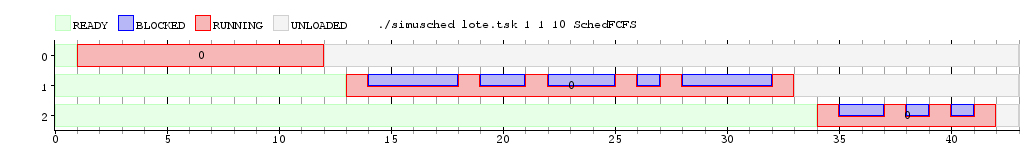
\includegraphics[scale=0.45]{../tp1/Test/resEj2Co1.png}
\\
\vspace{1pt}
\footnotesize\textit{Simulacro FCFS con un n\'ucleo}
\end{center}
\vspace{\baselineskip}


\vspace{\baselineskip}
\begin{center}
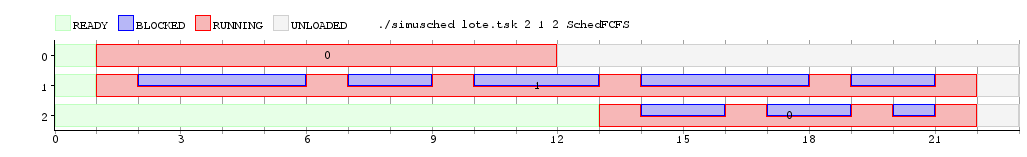
\includegraphics[scale=0.45]{../tp1/Test/resEj2Co2.png}
\\
\vspace{1pt}
\footnotesize\textit{Simulacro FCFS con dos n\'ucleos}
\end{center}
\vspace{\baselineskip}

\vspace{\baselineskip}
\begin{center}
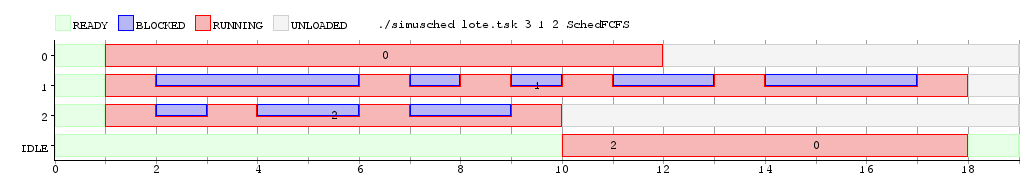
\includegraphics[scale=0.45]{../tp1/Test/resEj2Co3.png}
\\
\vspace{1pt}
\footnotesize\textit{Simulacro FCFS con tres n\'ucleos}
\end{center}
\vspace{\baselineskip}


Como podemos observar, los experimentos resultaron satisfactoriamente con nuestra hip\'otesis.

Adem\'as, notemos que en los casos en los que utilizamos la tarea TaskConsola, se observan claramente
las llamadas bloqueantes de manera random, dado que el tiempo tanto de la ejecuci\'on como el de las llamadas bloqueantes var\'ia.
En el caso en que el procesador tiene tres n\'ucleos, se observa que los n\'ucleos 2 y 0 ejecutan 
Idle ya que est\'an desocupadas, esperando la solicitud del pr\'oximo proceso.

\subsection{Ejercicio 3: Implementando Round-Robin}
La idea del scheduler \textit{Round-Robin} es darle un quantum a cada procesador, cuando un proceso lo solicita,
si alg\'un n\'ucleo esta desocupado, corre la tarea el tiempo que sea el quantum del procesador seleccionado.

Con esta idea desarrollamos nuestro Scheduler Round-Robin. Utilizamos como estructura una Cola $(q)$, para las llamadas a los procesos, 
un vector $(quantum)$ de tama\~no cantidad de cores del procesador que asignar\'a el quantum del i\'esimo n\'ucleo, 
y otro vector $(contador)$ que va a llevar cuenta del tiempo corrido por el proceso en el i\'esimo n\'ucleo hasta llegar al quantum del mismo.

Para el correcto funcionamiento en la funci\'on $tick$ se ven reflejados los casos en el cual el proceso debe 
dejar de correr ya sea porque termin\'o su tiempo o el quantum del procesador en el que corr\'ia. En \'este \'ultimo 
caso, la posici\'on correspondiente al n\'ucleo en $contador$ volver\'a a cero y el proceso se encolar\'a para terminar con su tiempo. 
\\Una vez realizada dicha acci\'on, debe dar lugar a la siguiente en la cola, o en caso de no haber una la Idle 
deber\'a hacerlo hasta el llamado de una nueva.

\subsection{Ejercicio 4: Experimentando Round-Robin}

En este ejercicio nos proponemos experimentar con el scheduler del punto anterior para verificar que el comportamiento es el esperado. Haremos esto de 
manera incremental, es decir, empezaremos probando las cosas mas basicas e iremos subiendo la complejidad. 

Para empezar, probaremos RR con un solo nucleo. Notese que si le asignamos una sola tarea, su comportamiento no diferiria de algun otro scheduler, por
lo que empezamos probando con cuatro tareas simultaneas. Estas tareas solo usan al cpu, por lo tanto no se bloquean. Esperamos 
verificar que el scheduler RR le asigna el tiempo del quantum a cada tarea antes de comenzar de nuevo la lista de tareas pendientes.

\vspace{\baselineskip}
\begin{center}
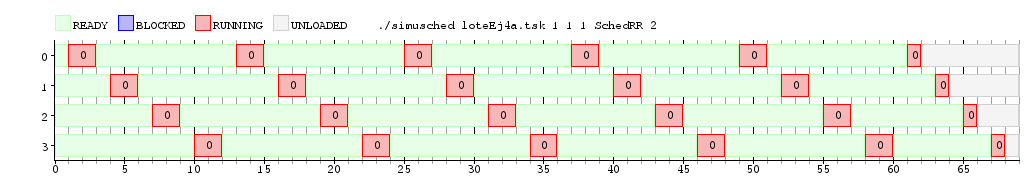
\includegraphics[scale=0.45]{../tp1/Test/resEj4Co1SB.png}
\\
\vspace{1pt}
\footnotesize\textit{Simulacro RR con un n\'ucleo}
\end{center}
\vspace{\baselineskip}

Efectivamente, cuando recibe k tareas simultaneas, el scheduler le asigna tiempo de ejecucion a las tareas de modo que todas 
ejecuten antes de regresar a ejecutar la primera. 

A continuacion usaremos el mismo lote de tareas, pero agregaremos otro procesador. Asi veremos si el scheduler maneja correctamente 
los procesadores para asegurarse que todas las tareas ejecuten un tiempo $quantum$ antes de volver a empezar.

\vspace{\baselineskip}
\begin{center}
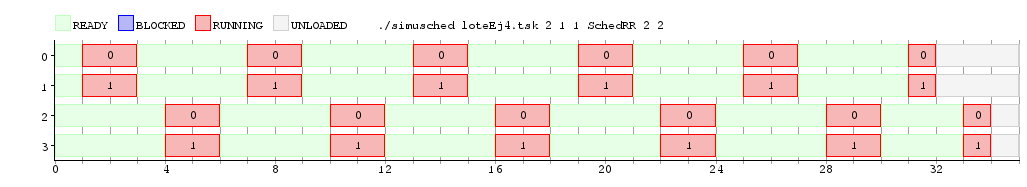
\includegraphics[scale=0.45]{../tp1/Test/resEj4Co2SB.png}
\\
\vspace{1pt}
\footnotesize\textit{Simulacro RR con dos n\'ucleo}
\end{center}
\vspace{\baselineskip}

El comportamiento es identico al anterior, solo que agregando otro nucleo, es decir, podemos deducir las mismas concluciones. Para probar de 
modo mas realista este scheduler, vamos a simular un lote de cuatro tareas que realicen llamadas bloqueantes, con dos procesadores para su ejecucion.
Lo que queremos mostrar, es que el scheduler trabajara de manera optima en este caso.

\vspace{\baselineskip}
\begin{center}
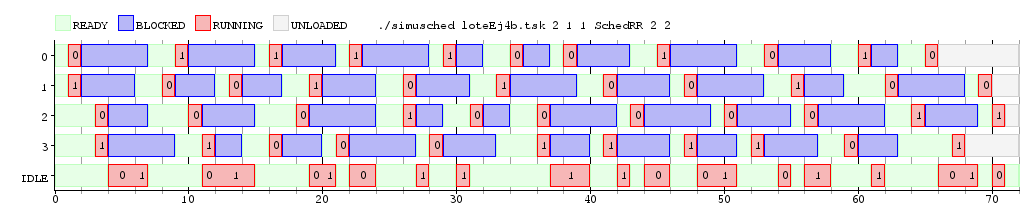
\includegraphics[scale=0.45]{../tp1/Test/resEj4Co2CB.png}
\\
\vspace{1pt}
\footnotesize\textit{Simulacro RR con dos n\'ucleo}
\end{center}
\vspace{\baselineskip}

Podemos ver que el scheduler trabaja de la manera esperada. Es decir, si hay un tarea disponible para ejecutar y procesador que no esta ejecutando nada,
ese procesador carga la tarea y la ejecuta, o bien hasta que se le acabe el quantum o hasta que se bloquee. Si todas las tareas estan bloqueadas 
o ejecutando cuando el procesador termina la ejecucion de una tarea porque se bloqueo, este se poner a ejecutar la tarea IDLE hasta que 
una tarea se desbloque. Y por lo tanto, si todas las tareas estan bloqueadas, ambos procesadores ejecutan la tarea IDLE hasta que alguna 
tarea se desbloquee.



\subsection{Ejercicio 5}
Este ejercicio est\'a dividido en dos incisos: en el primero, contestaremos una serie de preguntas formuladas por la c\'atedra, basando nuestras respuestas en el 
art\'iculo \textit{Scheduling algorithms for multiprogramming in a hard-real-time environment}; en el segundo, explicaremos el dise\~no e implementaci\'on 
de los algoritmos de scheduling de prioridades fijas y din\'amicas presentados en dicho art\'iculo.
\subsection*{Inciso 1}
En este inciso, debemos contestar tres preguntas te\'oricas acerca de los algoritmos de scheduling propuestos en el art\'iculo previamente mencionado. Antes de 
contestar las preguntas, comenzaremos con una breve descripci\'on de las condiciones de entorno sobre las cuales los algoritmos fueron ideados.
\newline
\newline
Se cuenta con un sistema, con un conjunto de tareas destinadas a resolver, cada una, una determinada funcionalidad vital para el correcto funcionamiento
de dicho sistema. Cada una de estas tareas estar\'a asociada a un evento externo, que solicitar\'a su ejecuci\'on. Es importante destacar que las tareas no
pueden ser ejecutadas antes de que dicho evento las solicite. Adem\'as, se sabe que cada tarea tiene, por un lado, una \textit{deadline} (esto es, una cantidad
de tiempo m\'aximo en el cual su ejecuci\'on debe terminar), que se mantendr\'a constante durante toda la ejecuci\'on del sistema. Por otro lado, se sabe
que el evento que solicitar\'a la ejecuci\'on de cada tarea, solicitar\'a peri\'odicamente (esto es, el intervalo de tiempo entre dos solicitudes ser\'a
siempre el mismo y no depender\'a de la terminaci\'on de otras tareas solicitadas) la ejecuci\'on de dicha tarea y, adicionalmente, se sabe que el tiempo de 
ejecuci\'on de cada tarea (entendiendo tiempo de ejecuci\'on como la cantidad de clocks que le llevar\'ia a una tarea comenzar y terminar su ejecuci\'on si el 
procesador s\'olo tuviera que ejecutar a esa tarea) ser\'a constante. Una condici\'on extra establece la existencia de tareas no peri\'odicas: estas tareas
desplazaran del procesador a las peri\'odicas y, a diferencia de las peri\'odicas, no tendr\'an una deadline estricta para terminar. Una vez establecidas
las condiciones del sistema, estamos listos para contestar las preguntas:
\newline
\newline
\textit{a}) \textquestiondown Qu\'e problema est\'an intentando resolver los autores?
\newline
\newline
Dado un sistema que se ajuste a las condiciones de entorno previamente explicadas, los autores quieren hallar una forma de organizar la ejecuci\'on de las
tareas, a medida que estas son solicitadas, de manera tal de que todas terminen su ejecuci\'on antes de su respectiva \textit{deadline}. Para esto, los 
algoritmos presentados estar\'an basados en prioridades (c\'omo se le asignar\'a la prioridad a cada tarea variar\'a seg\'un el algoritmo), y los algoritmos
de scheduling deber\'an, en cualquier momento, desalojar a la tarea que est\'e ocupando el procesador si llega una solicitud para la ejecuci\'on de una
tarea m\'as prioritaria, con lo cual, la clave para este tipo de algoritmos estar\'a en c\'omo se le asignar\'an las prioridades a las tareas.
\newline
\newline
\textit{b}) ?` Por qu\'e introducen el algoritmo de la secci\'on 7? ?`Qu\'e problema buscan resolver con esto?
\newline
\newline
Los autores introducen el algoritmo de la secci\'on 7, buscando bajar la cota superior de ln 2 sobre el tiempo de utilizaci\'on del procesador establecida 
por el algoritmo de scheduling con prioridades fijas, sin la necesidad de ninguna hip\'otesis extra los tiempos de ejecuci\'on de las tareas, ni tampoco 
necesitar relajar las \textit{deadlines} de las tareas menos prioritarias seg\'un el esquema anterior. Para lograr esto, introducen el algoritmo de 
scheduling con prioridades asignadas din\'amicamente; es decir, a lo largo de la ejecuci\'on del sistema, las prioridades de las tareas no estar\'an
necesariamente fijas.
\newline
\newline
\textit{c}) Explicar coloquialmente el significado del teorema 7.
\newline
\newline
El teorema 7 establece una condici\'on necesaria y suficiente, sobre el algoritmo de prioridades din\'amicas, para que todas las tareas terminen de ejecutarse
antes de su \textit{deadline}. Dicha condici\'on es la siguiente:

\begin{equation*}
 C_{1}/T_{1} + ... + C_{n}/T_{n} \leq 1
\end{equation*}

donde
\begin{itemize}
  \item $n:=$ n\'umero de tareas en el sistema
  \item $C_{i}:=$ tiempo de ejecuci\'on de la tarea i\'esima
  \item $T_{i}:=$ tiempo entre dos solicitudes consecutivas por la tarea i\'esima (tambi\'en llamado per\'iodo)
\end{itemize}

Es importante se\~nalar que la condici\'on que establece este teorema nos permitir\'a, dado un lote de tareas dise\~nado para nuestros experimentos, definir 
si el algoritmo de scheduling con propiedades din\'amicas lograr\'a que todas las tareas terminen de ejecutar antes de sus respectivas \textit{deadlines}, a lo 
largo de toda la simulaci\'on.

\subsection*{Inciso 2}

En este inciso explicaremos brevemente en qu\'e consiste cada algoritmo de scheduling, y luego el dise\~no y la implementaci\'on de cada uno.

El algoritmo de scheduling con prioridades fijas le asignar\'a a las tareas, como su nombre indica, una prioridad que se mantendr\'a fija a lo largo de 
toda la ejecuci\'on del sistema. Concretamente, una tarea ser\'a m\'as prioritaria que otra cuando su per\'iodo (el tiempo constante transcurrido entre
dos solicitudes por dicha tarea) sea menor o, lo que es equivalente, que su \textit{request rate}, definido como el inverso multiplicativo del per\'iodo,
sea mayor. Para el dise\~no de este algoritmo de scheduling, optamos por utilizar una cola de prioridad, que contendra duplas de la forma 
$<periodo(pid),pid>$, donde el m\'as prioritario ser\'a el que tenga menor per\'iodo. Este dise\~no nos permitir\'a obtener de manera sencilla cu\'al es
la pr\'oxima tarea a ser ejecutada, aprovechando las funcionalidades ya implementadas en la clase \textit{priority queue} para encolar elementos y obtener
el m\'as prioritario. De esta manera, obtener en cada tick de reloj cu\'al es la tarea a ejecutarse se resumir\'a a verificar, en primer lugar, si la 
cola de prioridad est\'a vac\'ia: en caso de que est\'e vac\'ia, se ejecutar\'a la tarea Idle, en caso contrario, se obtendr\'a el \textit{pid} de la 
pr\'{o}xima tarea a ser ejecutada mediante la funci\'on \textit{top()}, devolviendo el segundo componente de la dupla devuelta por dicha funci\'on.

El algoritmo de scheduling con prioridades din\'amicas, a diferencia del algoritmo anterior, le asignar\'a las prioridades a cada tarea en cada
\textit{tick} de reloj, haci\'endolo de la siguiente manera: a cada momento de la ejecuci\'on del sistema, la tarea m\'as prioritaria ser\'a la que
tenga su \textit{deadline} m\'as pr\'oxima; coloquialmente, esto quiere decir que lo m\'as urgente ser\'a lo m\'as prioritario. Para el dise\~no de
este scheduler, como deb\'iamos actualizar las prioridades en todos los \textit{ticks} de reloj, optamos por utilizar arreglos en vez de una cola de 
prioridad ya que, de utilizar una cola de prioridad, ser\'ia m\'as complicado iterar los procesos contenidos en la tabla para actualizar sus prioridades.
Por lo tanto, contaremos con los siguientes arreglos:

\begin{itemize}
  \item \textit{int deadline[totaltasks]} indicara, para la tarea i\'esima, cu\'anto tiempo le queda antes de su \textit{deadline} en $deadline[i]$. Para las tareas
  no peri\'odicas, adoptamos la convenci\'on de almacenar un -1 en esa posici\'on del arreglo.
  \item \textit{bool ready[total tasks]} indicar\'a, para la tarea i\'esima, si est\'a lista para correr o no.
\end{itemize}

Adicionalmente, implementaos la funcion \textit{int tareasready()}, que devolver\'a la cantidad de tareas en estado \textit{ready}.
Para obtener, en cada \textit{tick} de reloj, la pr\'oxima tarea a ejecutarse, implementamos una funci\'on de acuerdo a la siguiente l\'ogica:
Si est\'a corriendo una tarea no peri\'odica, seguir ejecutando esa. En caso contrario, verificar, en primer lugar, si hay alguna tarea
no peri\'odica en estado \textit{ready}. En caso de haberla, pasar a ejecutar esa; en caso contrario, buscar la m\'as tarea peri\'odica en estado
\textit{ready} cuya \textit{deadline} est\'e m\'as pr\'oxima, vali\'endonos para eso del arreglo \textit{deadline}, y devolver esa. Vale la pena aclarar
que adem\'as, en cada \textit{tick} de reloj, se decrementar\'a el valor contenido en el arreglo \textit{deadline} para cada tarea peri\'odica que est\'e
lista para ejecutarse. En este punto, hacemos la aclaraci\'on de que hemos dejado fuera de la descripci\'on algunos de los casos borde para los cuales no 
haya tareas listas para ejecutarse, en que deba devolverse el \textit{pid} de la tarea Idle, ya que no suma a la comprensi\'on del caso en que el algoritmo
deba buscar, entre las tareas existentes, la m\'as prioritaria.

\subsection{Ejercicio 6: TaskBatch}

En este ejercicio implementamos la tarea TaskBatch, que recibe como parametros totalcpu y cantbloqueos. Esta tarea dura totalcpu tiempo de 
cpu, y realiza cantbloqueos llamadas bloqueantes en momentos psudoaleatorios. Realizamos de dos maneras. La primera implementacion toma iteraba totalcpu
veces pidiendo un numero aleatorio rand. Si rand > 0.5 entonces llama a una tarea bloqueante, sino, a una tarea que use el cpu. Si la cantidad 
de iteraciones se acaba sin haber realizado todas las llamadas bloqueantes, entonces se realizaban las restantes seguidas al final. Sino, cuando se realizaba
la ultima llamada bloqueante, se utilizaba el tiempo restante del cpu todo junto. Lo que observamos en esta implementacion fue que las llamadas bloqueantes
se hacian para tiempos grandes siempre al principio del intervalo de uso del cpu, y para tiempos de medianos a cortos, siempre al final.**********

Por eso realizamos otra implementacion. En esta se seleccionan previamente en que momentos se van a realizar las llamadas bloqueantes, y luego se itera 
sobre el tiempo del cpu.


\subsection{Ejercicio 7}
\subsection{Ejercicio 8: Round Robin sin migracion}

En este ejercicio implementamos un scheduler Round Robin que no permite migraciones entre procesos. Para lograr esto, mantenemos una
cola por procesador 
y un contador que controla cuantas tareas hay activas por cpu. Para asignar una tarea a un cpu, nos basta con recorrer los contadores 
y quedarnos con alguno
de los de valor minimo. Ademas, cada vez que una tarea se bloquea, almacenamos en una variable cual
es el procesador al que estaba asignada. De este modo, para todos los procesadores, podemos ejecutar como si fuera Round Robin comun. La diferencia
radica en que cuando una tarea se bloquea, se almacena el valor de cpu de la misma. Cuando la tarea se desbloquea, basta con buscar su
cpu y pushearla en la cola del mismo.

Y los experimentos los tengo que pensar un ratito mas.

\subsection{Ejercicio 9}

En este ejercicio, debimos idear un lote de tareas que cumpliera en simult\'aneo, las siguientes condiciones:

\begin{itemize}
 \item Tener un scheduling no factible para el algoritmo de prioridades fijas
 \item Tener un scheduling factible para el algoritmo de prioridades din\'amicas
\end{itemize}

El lote que propusimos para este experimento es el siguiente:

\begin{verbatim}
  lote.tsk:
    &A1,10,4
    &B3,4,1
\end{verbatim}

Es decir, una repetici\'on de tarea de tipo A, con 4 ciclos de clock de tiempo de ejecuci\'on y 10 ciclos de clock como per\'iodo, y 3 repeticiones 
de tareas de tipo B, con 1 ciclo de clock de tiempo de ejecuci\'on y per\'iodo igual a 4. A continuaci\'on, mostraremos que con esta combinaci\'on
de per\'iodos y tiempos de ejecuci\'on, la tarea A no terminar\'a de ejecutarse antes de su \textit{deadline} (ciclo de clock n\'umero 10) 
para el scheduler de prioridades fijas. Es importante notar que a los tiempos de ejecuci\'on de las dos familias de tareas hay que sumarle el ciclo
de clock extra correspondiente a la llamada a \textit{exit()}, con lo cual, la tarea A requerir\'a de 5 ciclos para completar su ejecuci\'on, y las tareas 
B requerir\'an de 2 ciclos cada una.

Veamos el diagrama de Gantt para este lote, con scheduling con prioridades fijas:

\vspace{\baselineskip}
\begin{center}
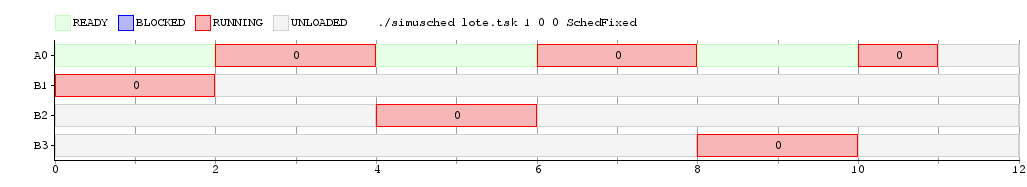
\includegraphics[scale=0.45]{../tp1/Test/ejercicio9-1.png}
\\
\vspace{1pt}
\footnotesize\textit{Simulaci\'on SchedFixed}
\end{center}
\vspace{\baselineskip}

En los instantes m\'ultiplos de 4 (0, 4 y 8) llega al sistema una \textit{request} por una tarea de familia B, mientras que en el instante 0 llega la \'unica 
\textit{request} por una tarea de tipo A. Como las tareas de tipo B, por tener menor per\'iodo, son m\'as prioritarias que la de tipo A, en los instantes
0, 4 y 8, el scheduler decide poner a correr las tareas de tipo B, durante los dos ciclos que necesitan para terminar. Esto le deja a la tarea A
4 ciclos de clock disponibles en los primeros 10 ciclos de clock, con lo cual no puede terminar la ejecuci\'on antes de que llegue su deadline,
haciendo inviable el uso del scheduler de prioridades fijas para este lote de tareas.
\\
Ejecutando el mismo lote de tareas, pero con scheduling de prioridades din\'amicas, obtenemos el siguiente diagrama de Gantt:

\vspace{\baselineskip}
\begin{center}
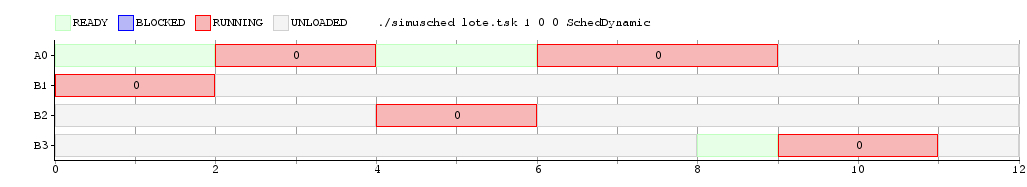
\includegraphics[scale=0.45]{../tp1/Test/ejercicio9-2.png}
\\
\vspace{1pt}
\footnotesize\textit{Simulaci\'on SchedDynamic}
\end{center}
\vspace{\baselineskip}

En esta simulaci\'on, el comportamiento del scheduler es id\'entico al de prioridades fijas hasta el instante 8, correspondiente a la tercer \textit{request}
por una tarea de tipo B. En este instante, la tarea de tipo A tiene su deadline dentro de 2 ciclos de clock, mientras que la tarea de tipo B tiene
su deadline a 4 ciclos de clock de distancia, por lo cual el scheduler decidir\'a poner a correr a la tarea de tipo A en vez de la tarea de tipo B.
Esto le permitir\'a a la tarea de tipo A consumir el \'ultimo ciclo de CPU que necesitaba, y luego el scheduler pondr\'a a correr a la \'ultima
tarea de tipo B, que terminar\'a sin problemas su ejecuci\'on. As\'i, todas las tareas del lote terminaron su ejecuci\'on antes de su \textit{deadline}.

\subsection{Ejercicio 10}